\documentclass[a4paper]{article}
\usepackage[margin=1in]{geometry}
\usepackage[operators]{cryptocode}
\usepackage{tikz}
\renewcommand\O[1]{\ensuremath{\mathsf{#1}}}
\newcommand{\M}[1]{\ensuremath{\text{\texttt{#1}}}}
\newcommand{\n}[1]{\ensuremath{\mathit{#1}}}
\tikzstyle{package} = [inner sep=1pt,align=center,rounded corners,draw,minimum width=2cm,minimum height=1cm,font=\small]
\tikzstyle{onarrow} = [inner sep=1pt,font=\scriptsize,anchor=east,at end,xshift=-0.1mm,align=left,fill=white]
%\title{Proof: Modularize}
\begin{document}
%\maketitle
\section{Games}
\subsection{monprfreal Game}
\begin{center}
\input{CompositionGraph_monprfreal.tex}
\end{center}
\begin{center}
\begin{pchstack}
\begin{pcvstack}\underline{\underline{\M{red}}}\\
\procedure{\O{Eval}(h)}{
\n{y} \stackrel{\mathsf{\tiny{invoke}}}{\gets} \O{Eval}(\n{h}) \pccomment{Pkg: prf} \\
\n{K}[\n{h}] \gets \O{some}(\n{y})
}
\pcvspace
\procedure{\O{Get}(h)}{
 \pcreturn \O{unwrap}(\n{K}[\n{h}])\\
}

\end{pcvstack}

\pchspace
\begin{pcvstack}\underline{\underline{\M{prf}}}\\\begin{pchstack}
\procedure{\O{Eval}(h)}{
\pcif \n{ltk} = \O{none}(\O{Bits("n")}) \pcthen\\
\pcind\n{ltk\_} \stackrel{1}{\sample} \O{Bits("n")}\\
\pcind \n{ltk} \gets \O{some}(\n{ltk\_})\\
 \pcreturn \O{prf}(\O{unwrap}(\n{ltk}), \n{h})\\
}
\pchspace
\end{pchstack}\end{pcvstack}

\end{pchstack}
\end{center}
\subsection{modprfreal Game}
\begin{center}
\input{CompositionGraph_modprfreal.tex}
\end{center}
\begin{center}
\begin{pchstack}
\begin{pcvstack}\underline{\underline{\M{mod\_prf}}}\\\begin{pchstack}
\procedure{\O{Eval}(h)}{
\pcif \n{ltk} = \O{none}(\O{Bits("n")}) \pcthen\\
\pcind\n{ltk\_} \stackrel{1}{\sample} \O{Bits("n")}\\
\pcind \n{ltk} \gets \O{some}(\n{ltk\_})\\
 \n{ltk\_} \gets \O{unwrap}(\n{ltk})\\
 \n{k} \gets \O{prf}(\n{ltk\_}, \n{h})\\
\n{\_} \stackrel{\mathsf{\tiny{invoke}}}{\gets} \O{Set}(\n{k}, \n{h}) \pccomment{Pkg: key}
}
\pchspace
\end{pchstack}\end{pcvstack}

\pchspace
\begin{pcvstack}\underline{\underline{\M{key}}}\\
%\begin{pchstack}
\procedure{\O{Set}(k, h)}{
\pcif \n{K}[\n{h}] = \O{none}(\O{Bits("n")}) \pcthen\\
\pcind \n{K}[\n{h}] \gets \O{some}(\n{k})
}
\pcvspace
\procedure{\O{Get}(h)}{
 \pcreturn \O{unwrap}(\n{K}[\n{h}])\\
}
%\pchspace
%\end{pchstack}
\end{pcvstack}

\end{pchstack}
\end{center}
%\subsection{monprfideal Game}
%\input{CompositionGraph_monprfideal.tex}
%\end{center}
%\begin{center}
%\begin{pchstack}
%\begin{pcvstack}\underline{\underline{\M{red}}}\\
\procedure{\O{Eval}(h)}{
\n{y} \stackrel{\mathsf{\tiny{invoke}}}{\gets} \O{Eval}(\n{h}) \pccomment{Pkg: prf} \\
\pcif \n{K}[\n{h}] = \O{none}(\O{Bits("n")}) \pcthen\\
\pcind \n{K}[\n{h}] \gets \O{some}(\n{y})\\
}
\pcvspace
\procedure{\O{Get}(h)}{
 \pcreturn \O{unwrap}(\n{K}[\n{h}])\\
}

\end{pcvstack}

%\pchspace
%\begin{pcvstack}\underline{\underline{\M{prf}}}\\\begin{pchstack}
\procedure{\O{Eval}(h)}{
\pcif \n{ltk} = \O{none}(\O{Bits("n")}) \pcthen\\
\pcind\n{ltk\_} \stackrel{1}{\sample} \O{Bits("n")}\\
\pcind \n{ltk} \gets \O{some}(\n{ltk\_})\\
 \pcreturn \O{prf}(\O{unwrap}(\n{ltk}), \n{h})\\
}
\pchspace
\end{pchstack}\end{pcvstack}

%\end{pchstack}
%\end{center}
%\subsection{modprfideal Game}
%\begin{center}
%\input{CompositionGraph_modprfideal.tex}
%\end{center}
%\begin{center}
%\begin{pchstack}
%\begin{pcvstack}\underline{\underline{\M{mod\_prf}}}\\\begin{pchstack}
\procedure{\O{Eval}(h)}{
\pcif \n{ltk} = \O{none}(\O{Bits("n")}) \pcthen\\
\pcind\n{ltk\_} \stackrel{1}{\sample} \O{Bits("n")}\\
\pcind \n{ltk} \gets \O{some}(\n{ltk\_})\\
 \n{ltk\_} \gets \O{unwrap}(\n{ltk})\\
 \n{k} \gets \O{prf}(\n{ltk\_}, \n{h})\\
\n{\_} \stackrel{\mathsf{\tiny{invoke}}}{\gets} \O{Set}(\n{k}, \n{h}) \pccomment{Pkg: key}
}
\pchspace
\end{pchstack}\end{pcvstack}

%\pchspace
%\begin{pcvstack}\underline{\underline{\M{key}}}\\
%\begin{pchstack}
\procedure{\O{Set}(k, h)}{
\pcif \n{K}[\n{h}] = \O{none}(\O{Bits("n")}) \pcthen\\
\pcind \n{K}[\n{h}] \gets \O{some}(\n{k})
}
\pcvspace
\procedure{\O{Get}(h)}{
 \pcreturn \O{unwrap}(\n{K}[\n{h}])\\
}
%\pchspace
%\end{pchstack}
\end{pcvstack}

%\end{pchstack}
%\end{center}
\section{Equivalence between modprfreal and monprfreal}
\scalebox{0.7}{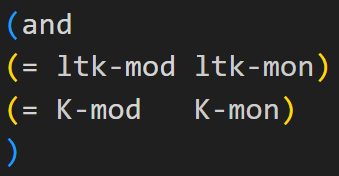
\includegraphics{invariant-code.png}}
\scalebox{0.7}{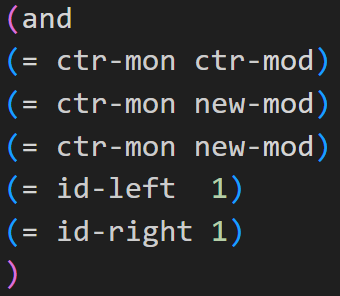
\includegraphics{randomness-mapping.png}}
\scalebox{0.7}{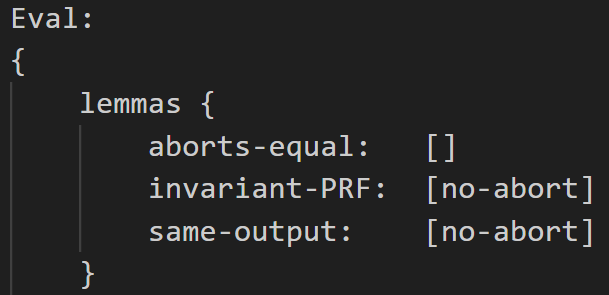
\includegraphics{lemmas.png}}

\noindent
We need to define an invariant on the states of the two games (left), namely that the two games have the same content in table $K$ and variable $\mathsf{ltk}$. We need a randomness relation (middle), namely, that the two games use the same randomness to sample $\mathsf{ltk}$. Then, the SMT solver tries to prove the three core lemmas (right) for us, namely that invariant implies equal aborts, and, if there are no aborts, then the invariant holds again after the call and the outputs are equal.

%\section{Equivalence between modprfreal and monprfreal}
\end{document}






